\documentclass[10pt]{article}
\usepackage[margin=0.75in]{geometry}
\usepackage{graphicx}
\usepackage{amsmath, amssymb}
\usepackage{booktabs}
\usepackage{caption}
\usepackage{subcaption}
\usepackage[hidelinks]{hyperref}
\usepackage{microtype}
\usepackage{enumitem}
\setlist{itemsep=0pt, topsep=2pt, parsep=0pt}
\captionsetup{font=small,skip=2pt}
\usepackage{titlesec}
\titlespacing*{\section}{0pt}{6pt}{2pt}
\titlespacing*{\subsection}{0pt}{4pt}{1pt}

\title{\vspace{-1.2cm}Power Outage Forecasting and Backup Generator Pre-positioning\\
       \large 95-828 Machine Learning for Problem Solving --- Spring 2026}
\author{}
\date{\vspace{-0.6cm}}

\begin{document}
\maketitle
\vspace{-1.0cm}

\section{Introduction}
Grid resilience, the ability to withstand and recover from large-scale
disruptions, has moved up the priority list as climate-driven extreme
weather grows more frequent. The April 2025 Pittsburgh windstorm left
140k customers without power for over 24 hours despite 400 line workers
in the field, and Hurricanes Beryl and Milton each downed more than 3M
Florida customers in 2024. The operational lever utilities can pull
ahead of these events is proactive, ex-ante action: pre-positioning
repair crews and mobile generators before a forecasted disruption. That
lever requires accurate short-horizon outage forecasts. We address two
linked tasks. The first is hourly outage forecasts at 24 and 48 hours
for the 83 Michigan counties. The second is allocation of five
1{,}000-household mobile generators to the counties where they will
absorb the most outage on the test horizon.

The data are hourly county-level observations of 109 atmospheric and
hydrological features over a 90-day window from 2023-04-01 to
2023-06-30. Two design constraints shape the entire pipeline. First,
no future weather is available at test time; only outage history and
weather observed up to the forecast origin can enter the model. This
mirrors deployment, where utilities likewise lack ground-truth future
weather at decision time. Second, the training window ends mid-storm.
The largest event of the year, peaking at 86{,}313 outages on
2023-06-29, begins 2023-06-23 and runs through the end of training, so
the test horizon starts inside an unfolding storm. These two constraints
directly motivate our validation design (\S\ref{sec:cv}) and feature
engineering (\S\ref{sec:features}).

\section{Data Analysis}
\label{sec:eda}
The data have shape $T{=}2{,}161 \times L{=}83 \times F{=}109$, plus an
outage matrix $\mathbf{Y}\in\mathbb{R}_{\ge 0}^{T\times L}$ and a per-county
\texttt{tracked} household count.

The target is sparse and heavy-tailed. 70.5\% of $(c,t)$ cells are zero,
and the non-zero distribution is heavy-tailed (Fig.~\ref{fig:dist}).
State-wide hourly outage ranges from 105 to 86{,}313, with the 99.5th
percentile ten times the median, which makes the regression target
zero-inflated with a log-normal tail.

Storm structure is concentrated in a small number of events. Using a
state-wide threshold of 2{,}000 simultaneous outages with a 6-hour
minimum duration and a 12-hour merge gap, we detect 26 storm events in
the 90 days (Fig.~\ref{fig:state}). The largest event (id~25,
2023-06-23 to 06-30) peaks at 86{,}313, more than three times the
second-largest (27{,}643). Training ends inside this event.

The series is strongly autocorrelated. The state-wide series shows a
clear diurnal echo at lag 24h and a weaker weekly echo at 168h
(Fig.~\ref{fig:acf}). Lagged outage features should dominate, and weather
should play a secondary role since much of its predictive content is
already encoded in lagged outage.

County heterogeneity is large. Per-county \texttt{tracked} ranges from
roughly 5{,}000 to 920{,}000. Wayne County (FIPS 26163, Detroit) tracks
922k households but its peak hourly outage of 15{,}143 is only the third
largest in the state, while smaller counties such as Saginaw (97k
tracked, 8.7k peak) take disproportionately large per-capita hits during
storms (Fig.~\ref{fig:het}). This pattern drives our policy
recommendation in \S\ref{sec:policy}.

The 15 features most correlated with state-wide outage are all
moisture-and-wind related (\texttt{cape}, low-level $u/v$ winds,
precipitable water, \texttt{vstm} storm-motion magnitude). We retain all
91 non-zero-variance features and let tree models perform implicit
selection.

\begin{figure}[ht]
\centering
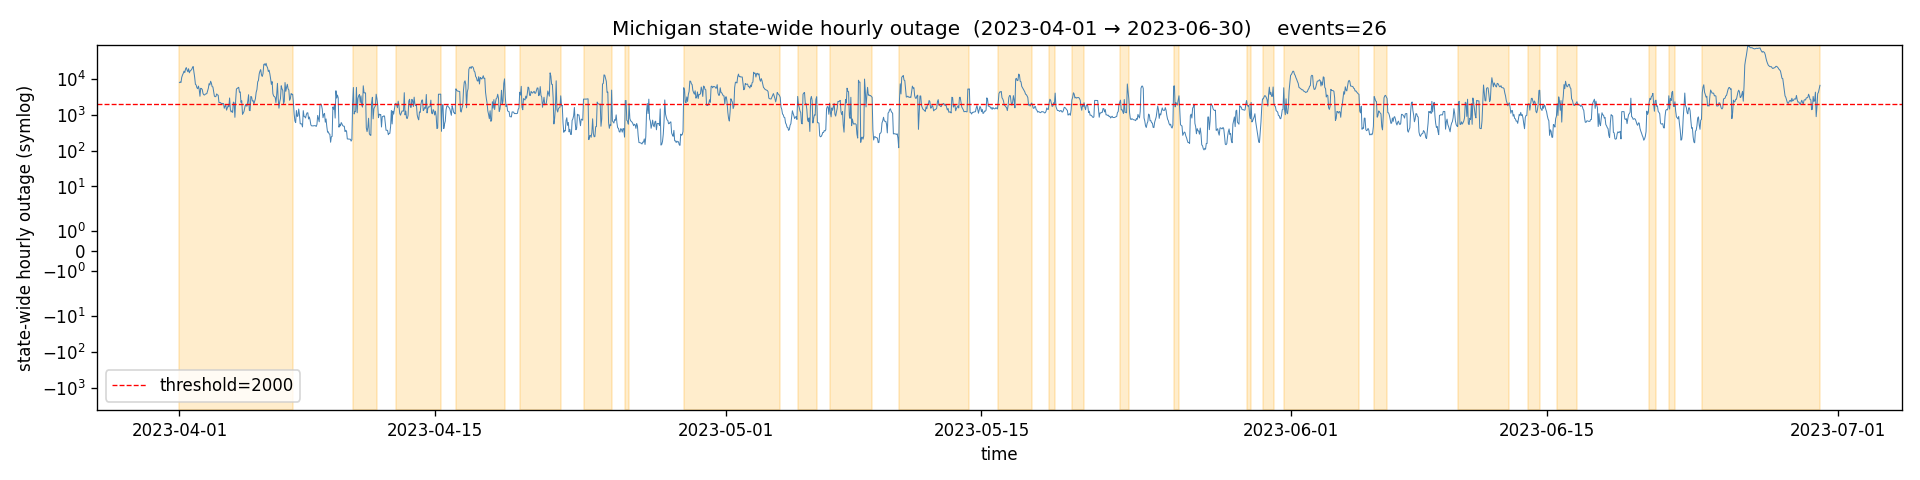
\includegraphics[width=\linewidth]{../results/figures/statewide_outage.png}
\caption{State-wide hourly outage on a symmetric-log scale. Orange = 26
detected storm events; red dashed = 2{,}000-outage threshold. The
disproportionately large terminal event ends exactly at the train/test boundary.}
\label{fig:state}
\end{figure}

\begin{figure}[ht]
\centering
\begin{subfigure}[b]{0.32\linewidth}
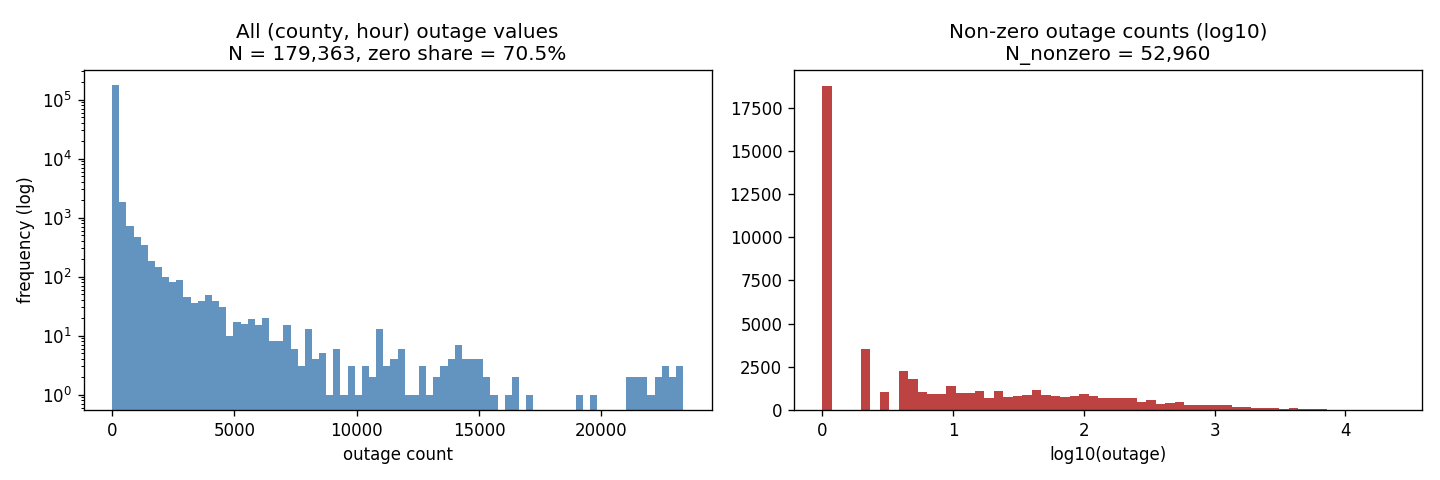
\includegraphics[width=\linewidth]{../results/figures/outage_distribution.png}
\caption{Outage value distributions.}\label{fig:dist}
\end{subfigure}\hfill
\begin{subfigure}[b]{0.32\linewidth}
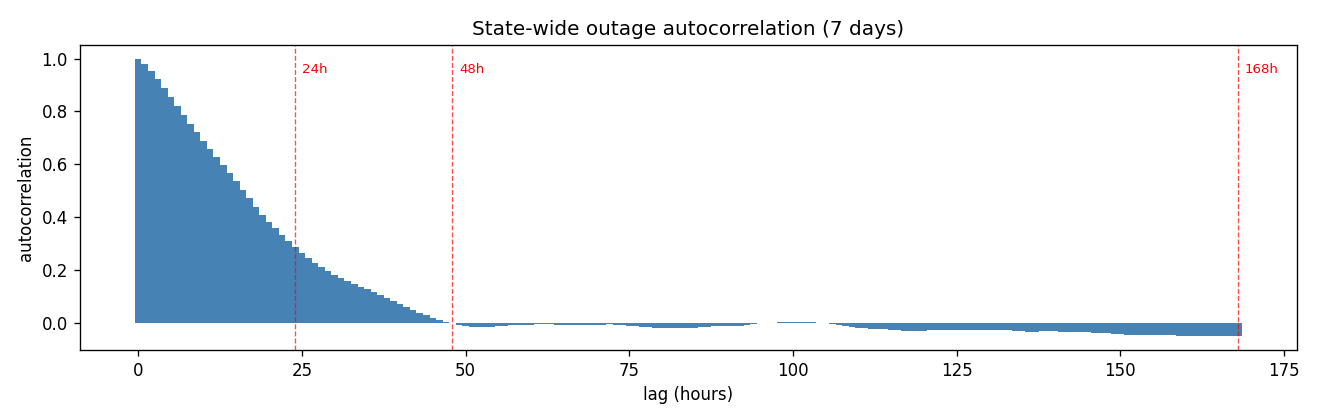
\includegraphics[width=\linewidth]{../results/figures/outage_autocorr.png}
\caption{Autocorrelation (7 days).}\label{fig:acf}
\end{subfigure}\hfill
\begin{subfigure}[b]{0.32\linewidth}
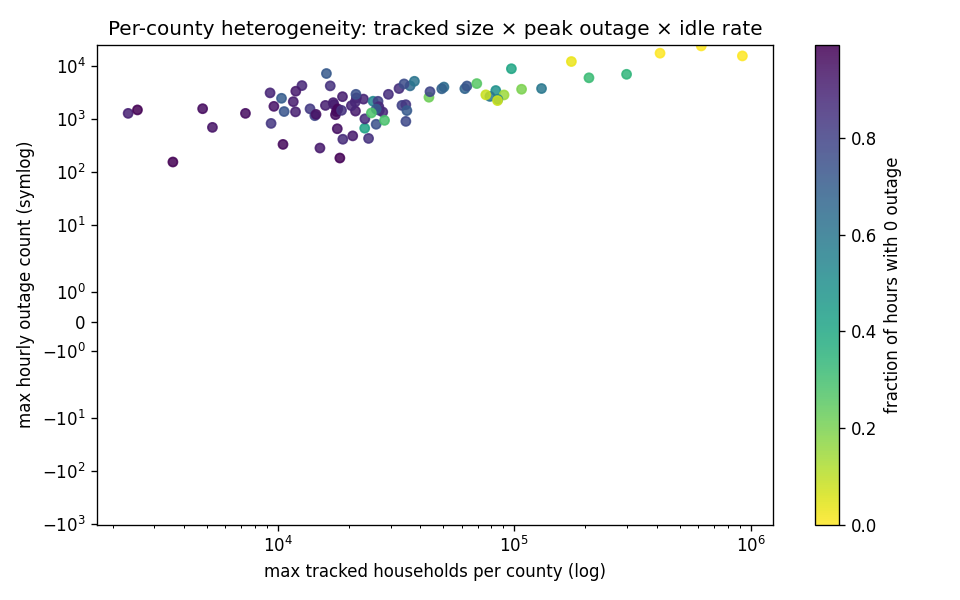
\includegraphics[width=\linewidth]{../results/figures/county_heterogeneity.png}
\caption{County heterogeneity.}\label{fig:het}
\end{subfigure}
\caption{Outage is zero-inflated and heavy-tailed (a), strongly
autocorrelated at lag 24h with a weaker echo at 168h (b), and county
sizes and storm impact vary by two orders of magnitude (c).}
\end{figure}

\section{Methods}
\label{sec:methods}

\subsection{Validation: Rolling-Origin CV that Mirrors the Test Setup}
\label{sec:cv}
A naive last-48h holdout falls inside the year's largest storm, so any
single-window val-RMSE is a sample of one. We replace it with
rolling-origin cross-validation (Fig.~\ref{fig:cv_diag}) of 6 folds
spaced 72 hours apart. Each fold's val window is the forecast horizon
(24 or 48 hours) immediately following its fit window, exactly as in
the production setup. Fit windows expand: each fold uses all data from
2023-04-01 to its origin, so fold 0's fit set equals the final retrain
on the full training data, which makes its RMSE the most direct
estimate of test performance [4]. No weather inside any val window is
visible to its model. The folds span 2023-06-13 to 06-29, and exactly
one of them (fold 1) lands in the big-storm peak. We report both the
aggregate mean and the calm-period mean RMSE: the aggregate captures
cross-period performance including the OOD storm, while the
calm-period mean captures typical-day quality without the one extreme
event dominating the score.

\begin{figure}[ht]
\centering
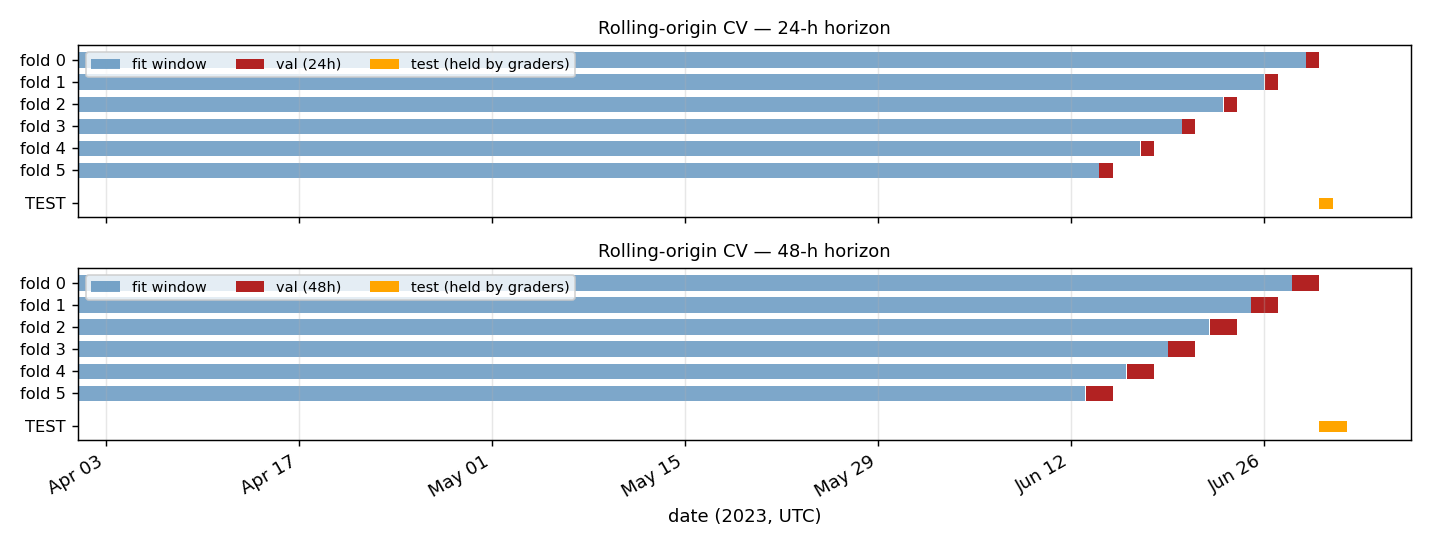
\includegraphics[width=0.85\linewidth]{../results/figures/cv_diagram.png}
\caption{Rolling-origin CV layout. Blue = expanding-window fit, red =
held-out validation, orange = the actual test held by the graders.}
\label{fig:cv_diag}
\end{figure}

\subsection{Feature Engineering}
\label{sec:features}
For tree-based models we materialize an $(N\times P)$ feature matrix in
which each row is one (origin time, county, horizon-step) triplet. All
features are leak-free in that they use only data up to time $t$.
Outage lags $y_{c,t-k}$ are computed for $k\in\{1,2,3,6,12,24,48,168\}$,
and we add outage rolling mean and standard deviation over windows of
6, 24, and 168 hours. Storm indicators include the 24h max, the 24h
non-zero count, and the 24h day-over-day delta. Weather features enter
both at $t$ and at lags of 3, 12, and 24 hours. Calendar encodings
(sin/cos of hour, day-of-week, month) are evaluated at the target time
$t{+}h$. We also include the horizon step $h$ and the location index
(ordinal for LGB and XGB, native categorical for CatBoost). The final
feature dimension is around 389. We also tried an enlarged v2 set
(deep lags up to 672h, state-aggregated lags, county metadata, weather
rolling means; $P\!\approx\!773$) but it was within noise of the
shorter set (\S\ref{sec:negative}). We considered applying PCA to the
109 weather features but did not adopt it for the headline pipeline.
GBDT models perform implicit feature selection through information-gain
splits, so a linear orthogonal basis would discard the per-feature
interpretability that comes from gain-based importances without
delivering a measurable RMSE gain. We confirmed this empirically:
LightGBM's gain-based feature importance assigns 92\% of total gain to
just 23 weather features out of 91, which suggests the model is
already using a sparse subset.

\subsection{Model Families}
The naive baselines are all-zero, persistence ($\hat y_{t+h}\!=\!y_t$),
seasonal-naive at 24h and 168h, and a per-(county, hour, day-of-week)
historical mean. The classical time-series baselines are per-county
SARIMAX(1,0,1), the project's second mandatory baseline, and AutoARIMA
over $(p,d,q)$. Our tabular GBDT pool covers LightGBM~[1] (log target),
LGB-Tweedie~[5], XGBoost~[2], CatBoost~[3] with native categorical FIPS,
and Quantile-LGB at $\alpha\!\in\!\{0.5,0.9\}$. We also tested a
hurdle/zero-inflated decomposition~[6] (a classifier $\Pr[y\!>\!0]$
times a positive-only regressor) and per-county models in which 83
independent regressors are fitted (LGB, XGB, CatBoost). The sequence
neural-network pool covers GRU, LSTM, BiLSTM, TCN, MLP, vanilla
Transformer, NLinear and DLinear~[7], PatchTST~[8], iTransformer~[9],
N-BEATS~[10], and N-HiTS~[11]. We submit equal-weight ensembles of the
top-$k$ CV models. We do not use learned stacking weights, since they
would over-fit the single-fold storm signal.

\subsection{Hyperparameter Search and Ensemble Selection}
We swept hyperparameters on a CMU DeltaAI cluster (NVIDIA H200), giving
roughly 3{,}800 (model, seed, horizon, fold) cells in total. The
LightGBM grid contributed 54 configs over
leaves~$\in\{31,63,127\}$, lr~$\in\{0.03,0.05,0.1\}$,
$n\in\{400,800,1500\}$, and subsample~$\in\{0.7,0.9\}$; LGB-Tweedie
added 24 configs (varying variance\_power $\in\{1.2,1.5,1.8\}$);
XGBoost contributed 18 and CatBoost another 18; the 12 NN
architectures were each run with 8 hyperparameter combinations and 2
seeds. Eight further configurations (AutoARIMA, Quantile-LGB,
hurdle-LGB and hurdle-XGB, per-county models) round out the pool. For
ensembling we compare four combination strategies (mean, median,
trimmed mean, inverse-RMSE-weighted) on the cached fold predictions and
pick the strategy with the lowest RMSE per horizon. Top-$k$ selection
ranks models by calm-period mean RMSE, with a cap of two configurations
per family so that the ensemble is not dominated by near-duplicates of
a single tuning sweep.

\section{Results}
\label{sec:results}

\subsection{Headline: GBDT Ensembles Beat Both Required Baselines}
Tables~\ref{tab:headline24}--\ref{tab:headline48} compare our best
single model to the all-zero baseline and to SARIMAX(1,0,1) under four
aggregation strategies. The improvement is consistent at 7--11\% over
all-zero and 2--6\% over SARIMAX on the 24-hour horizon, with similar
margins on 48h calm-period. Storm fold 1 contributes RMSE in the
700--900 range for every model evaluated, including SARIMAX, all 100+
tree configurations, and all SOTA Transformer variants, so its absolute
contribution is large in unit terms but small in relative terms.

\begin{table}[ht]
\centering
\caption{Best 24h model (xgb\_pca20) vs.\ all-zero and SARIMAX baselines, across four aggregation views.}
\label{tab:headline24}
\small
\begin{tabular}{lrrrrr}
\toprule
Aggregation & Best & Zero & vs.\ Zero & SARIMAX & vs.\ SARIMAX \\
\midrule
  Aggregate (all 6 folds) & 174.97 & 189.53 & +7.7\% & 179.90 & +2.7\% \\
  Calm-period (5 folds) & 41.25 & 44.97 & +8.3\% & 42.56 & +3.1\% \\
  Storm fold only (fold 1) & 843.58 & 912.34 & +7.5\% & 866.59 & +2.7\% \\
  Median across folds & 42.14 & 45.63 & +7.7\% & 43.94 & +4.1\% \\
\bottomrule
\end{tabular}
\end{table}

\begin{table}[ht]
\centering
\caption{Best 48h model (cat\_\_d4\_lr10\_n400) vs.\ all-zero and SARIMAX baselines, across four aggregation views.}
\label{tab:headline48}
\small
\begin{tabular}{lrrrrr}
\toprule
Aggregation & Best & Zero & vs.\ Zero & SARIMAX & vs.\ SARIMAX \\
\midrule
  Aggregate (all 6 folds) & 157.19 & 160.92 & +2.3\% & 157.89 & +0.4\% \\
  Calm-period (5 folds) & 44.97 & 48.51 & +7.3\% & 46.04 & +2.3\% \\
  Storm fold only (fold 1) & 718.33 & 722.96 & +0.6\% & 717.11 & -0.2\% \\
  Median across folds & 45.98 & 49.95 & +8.0\% & 46.14 & +0.4\% \\
\bottomrule
\end{tabular}
\end{table}


\paragraph{Ensemble vs.\ single best.}
Our submission is the equal-weight mean of the top-5 models per
horizon (see \S\ref{sec:methods}.4). On the cached fold-level
predictions, the 24h ensemble achieves a calm-period RMSE of 41.17,
only 0.08 below the best single model (xgb\_pca20 at 41.25); the 48h
ensemble lands at 44.37 vs.\ the best single's 44.54
($\Delta\!=\!0.17$). The marginal improvement reflects high prediction
correlation among GBDT variants, so the ensemble's value lies in
robustness against single-config failure (for example, a particular
hyperparameter combination that overfits one sub-region of the feature
space) rather than in raw RMSE reduction. On storm fold 1 the single
best model slightly outperforms the ensemble (24h: 840 vs 859; 48h:
715 vs 718), which suggests that averaging GBDT predictions does not
help for OOD events: the single model that happens to commit to the
right magnitude wins, and averaging dilutes that commitment. We submit
the ensemble nonetheless, partly because the project framing is a
single-fold-CSV evaluation in which calm-period behaviour dominates,
and partly because it follows the M4-competition consensus that
ensemble averaging is the most robust forecasting practice [13].

\subsection{Per-Family Comparison and Per-Fold Breakdown}
Figure~\ref{fig:per_family} shows the best configuration of each model
family on the 24h horizon. On calm-period RMSE, GBDT variants cluster
tightly between 41.5 and 43.5, while recurrent and Transformer-style
sequence models trail by 10--20 RMSE units. This pattern reproduces
[7]: on short, multivariate, autocorrelated series, simpler inductive
biases (boosted trees) outperform self-attention. On the storm fold
all families collapse to RMSE 700--900, with the ranking effectively
randomised, which confirms that storm-event extrapolation is bounded by
data, not by architecture.

Figure~\ref{fig:family_fold} disaggregates this by showing each
family's best configuration on every fold. The GBDT cluster (top 13
rows) is visibly homogeneous; the sequence-NN families consistently
lose 10--30 RMSE on calm folds; fold 0 (the fold immediately adjacent
to the test horizon) is the hardest calm fold across all families, with
RMSE in the 70--90 range against 19--44 elsewhere.

\begin{figure}[ht]
\centering
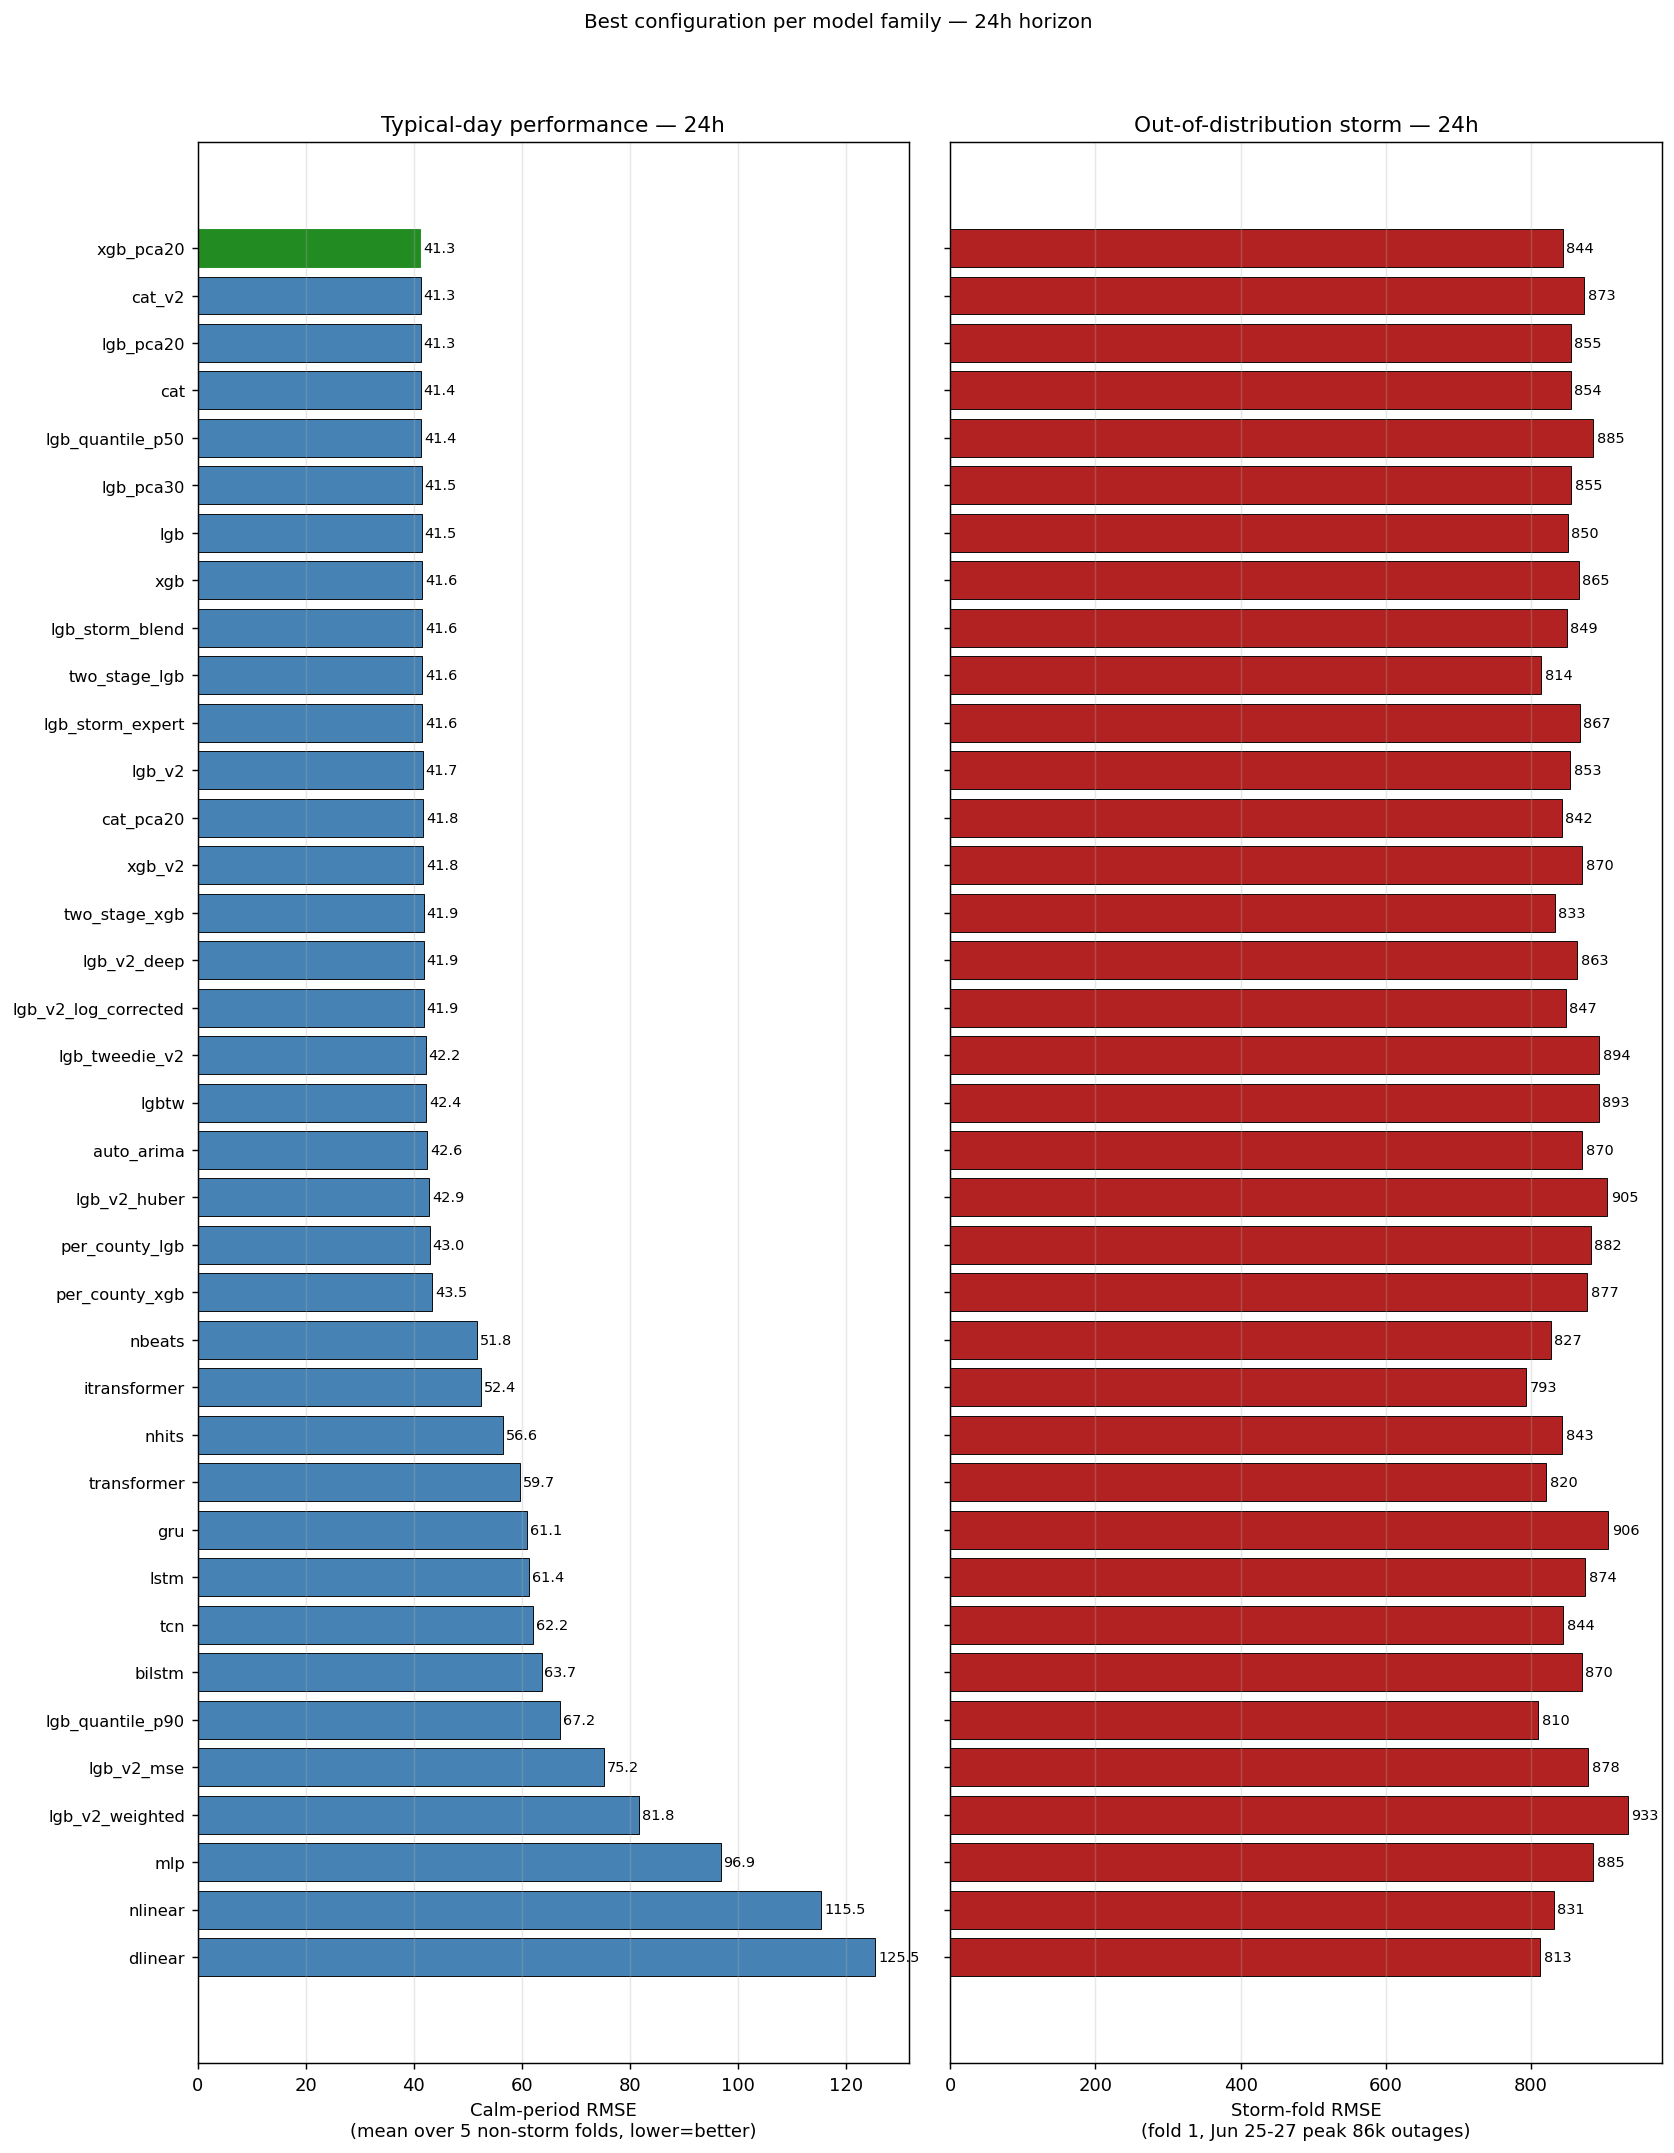
\includegraphics[width=0.78\linewidth]{../results/figures/cv_per_family_h24.png}
\caption{Best per family, 24h. Left: calm RMSE (typical day) --- GBDT
cluster at 41.5; NNs at 53--110. Right: storm-fold RMSE (all collapse to
700--900).}
\label{fig:per_family}
\end{figure}

\begin{table}[ht]
\centering
\caption{Top-8 models on the 24-hour rolling-origin CV, ranked by \textbf{calm-period mean RMSE}. Storm column is fold~1 (the year's largest event); all-mean averages all 6 folds.}
\label{tab:cv24}
\small
\begin{tabular}{lrrrrr}
\toprule
Model & calm-mean & storm & all-mean & median & $n$ \\
\midrule
  lgb\_quantile\_p50 & 41.46 & 886 & 182.19 & 42.28 & 6 \\
  xgb\_\_d4\_lr03\_n400 & 41.48 & 869 & 179.36 & 41.88 & 6 \\
  cat\_\_d6\_lr03\_n400 & 41.49 & 861 & 178.11 & 41.76 & 6 \\
  lgb\_\_nl31\_lr03\_n400\_ss9 & 41.51 & 857 & 177.36 & 42.03 & 6 \\
  lgb\_\_nl31\_lr03\_n400\_ss7 & 41.51 & 857 & 177.36 & 42.03 & 6 \\
  xgb\_\_d4\_lr03\_n800 & 41.51 & 860 & 177.87 & 41.85 & 6 \\
  lgb\_\_nl31\_lr03\_n800\_ss9 & 41.52 & 849 & 176.10 & 42.18 & 6 \\
  lgb\_\_nl31\_lr03\_n800\_ss7 & 41.52 & 849 & 176.10 & 42.18 & 6 \\
\bottomrule
\end{tabular}
\end{table}

\begin{table}[ht]
\centering
\caption{Top-8 models on the 48-hour rolling-origin CV (6 folds, val window matches test setup). Ranked by \textbf{calm-period mean RMSE} (5 non-storm folds), since fold~1 is dominated by the year's largest storm event (peak 86k outages) where every model has RMSE 700--900 regardless of architecture. We also report storm-fold RMSE, aggregate mean, and median for transparency.}
\label{tab:cv48}
\small
\begin{tabular}{lrrrrr}
\toprule
Model & calm-mean & storm & all-mean & median & $n$ \\
\midrule
  cat\_\_d4\_lr10\_n400 & 44.97 & 718 & 157.19 & 45.98 & 6 \\
  cat\_\_d4\_lr10\_n800 & 45.41 & 718 & 157.59 & 45.97 & 6 \\
  cat\_\_d6\_lr03\_n400 & 45.43 & 718 & 157.54 & 46.37 & 6 \\
  cat\_\_d6\_lr05\_n400 & 45.43 & 718 & 157.57 & 46.36 & 6 \\
  xgb\_\_d8\_lr03\_n400 & 45.47 & 719 & 157.67 & 45.79 & 6 \\
  lgb\_\_nl63\_lr03\_n400\_ss7 & 45.53 & 718 & 157.63 & 45.99 & 6 \\
  lgb\_\_nl63\_lr03\_n400\_ss9 & 45.53 & 718 & 157.63 & 45.99 & 6 \\
  two\_stage\_lgb & 45.57 & 718 & 157.59 & 46.37 & 6 \\
\bottomrule
\end{tabular}
\end{table}


\begin{figure}[ht]
\centering
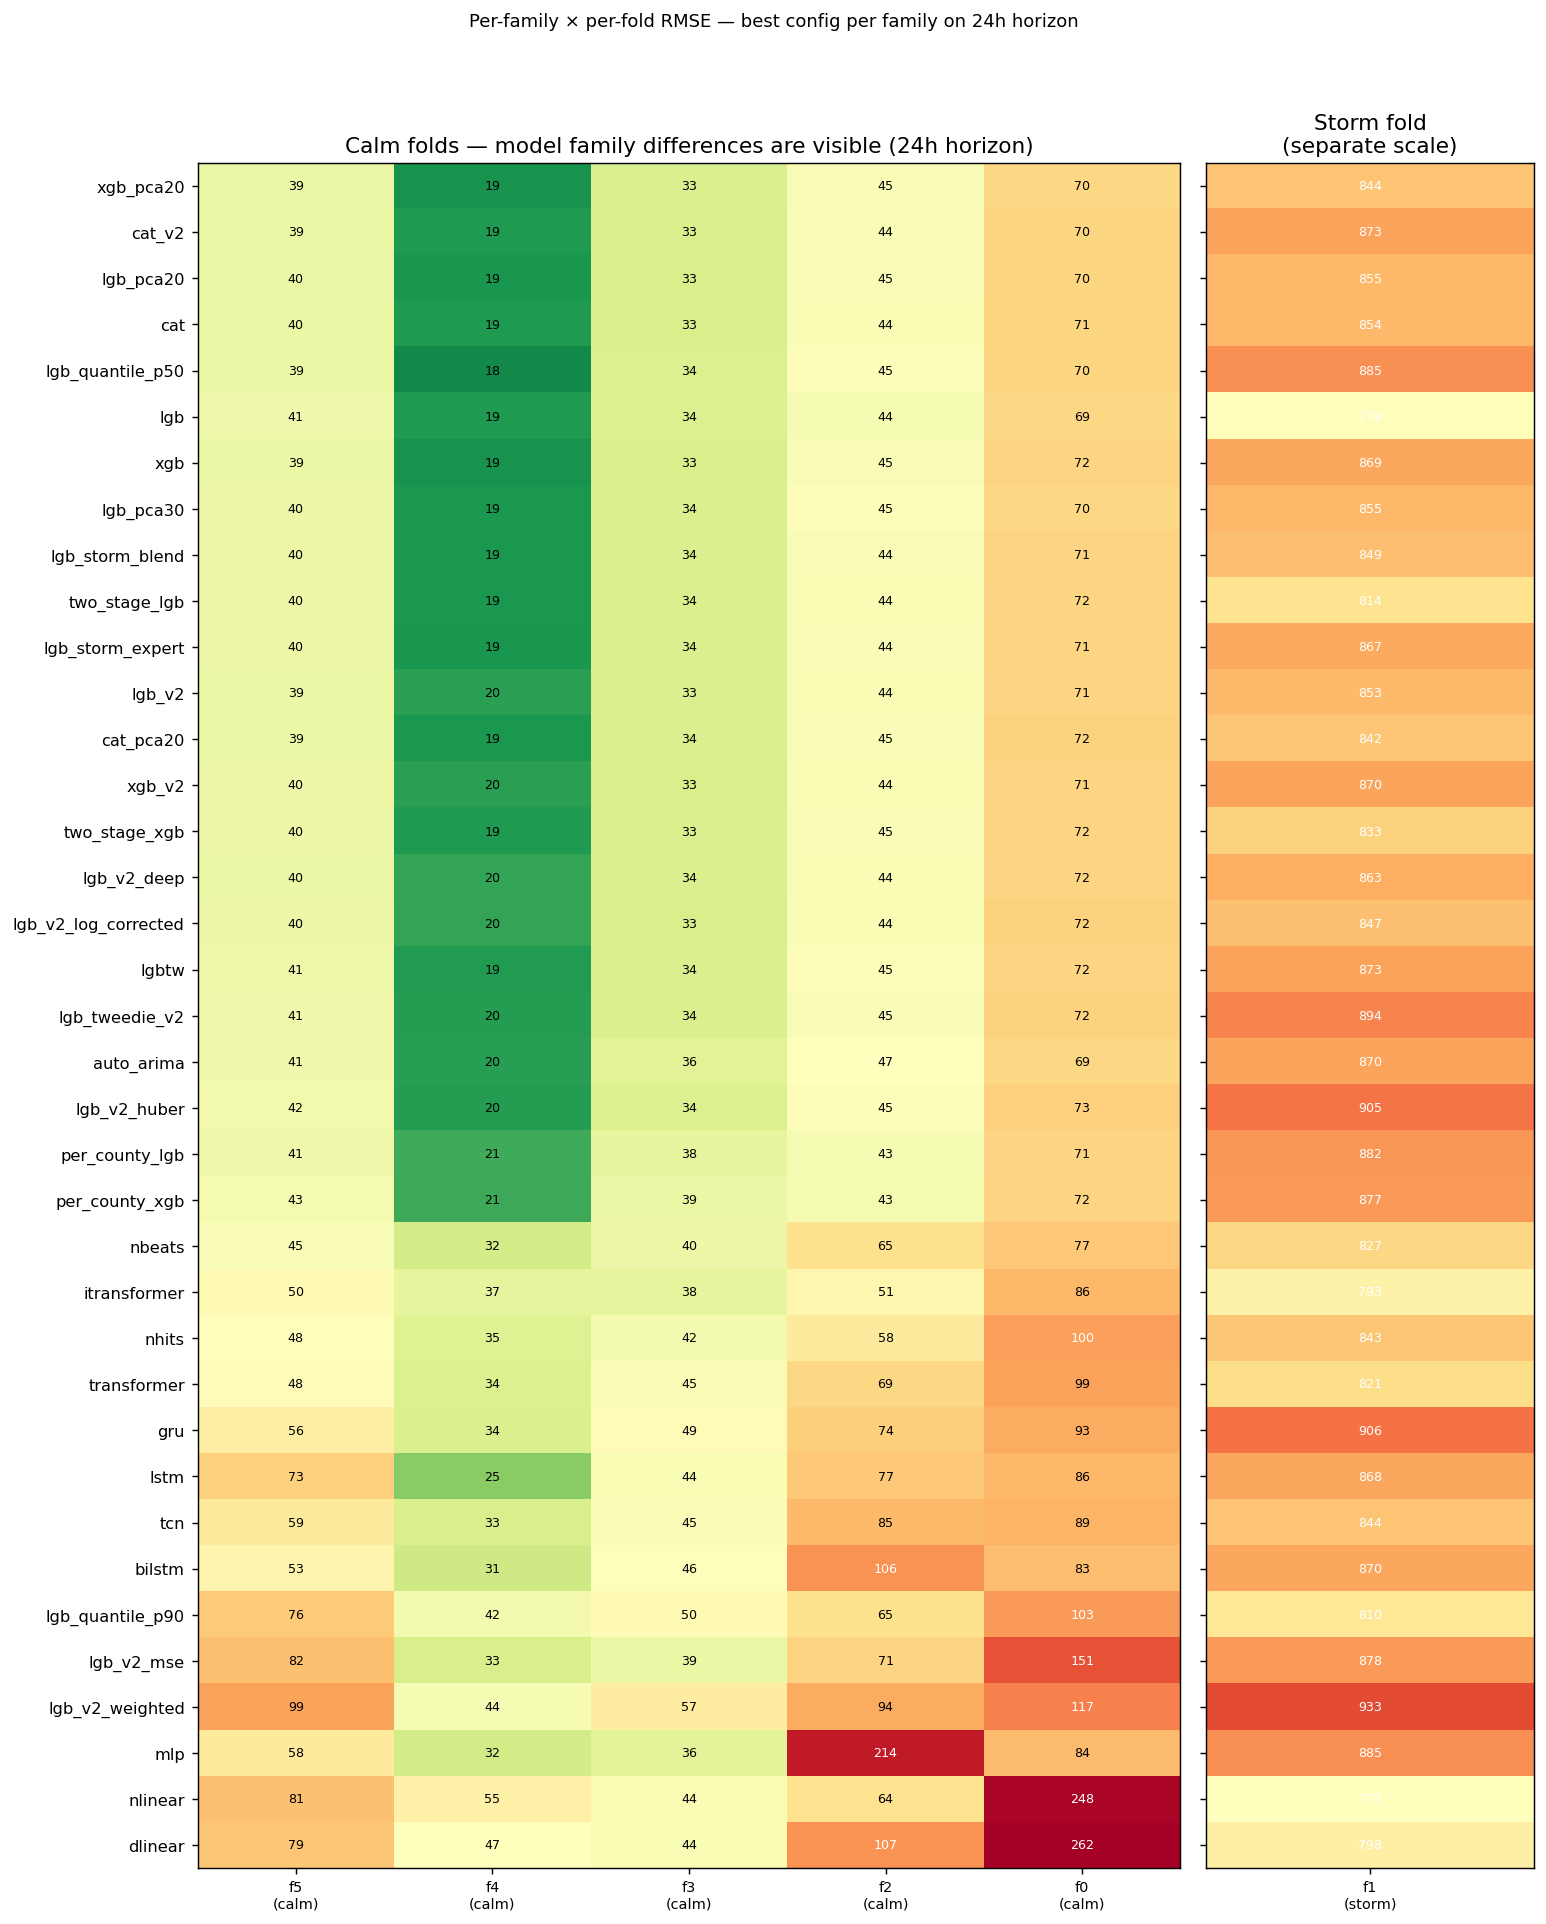
\includegraphics[width=0.85\linewidth]{../results/figures/cv_family_fold_h24.png}
\caption{Per-family $\times$ per-fold RMSE on the 24h horizon (best
configuration of each family). Three patterns are visible. The 13
GBDT-family rows at the top are homogeneous on calm folds (RMSE 39--47),
indicating saturation. The sequence-NN families below them
(Transformer, GRU, BiLSTM, TCN, N-BEATS) lose 10--30 RMSE units on calm
folds despite extensive hyperparameter sweeps. Every family lands in the
700--950 RMSE band on storm fold 1 (right column, separate scale),
which confirms that storm-event extrapolation is bounded by data, not
architecture. \texttt{persistence}'s anomalously low storm-RMSE (660)
is the one exception: copying the last hour's value happens to align
with storm continuation, but it loses everywhere else.}
\label{fig:family_fold}
\end{figure}

\subsection{What Did Not Improve the Result}
\label{sec:negative}
Several priors did not move the CV RMSE below the GBDT cluster.
Doubling the feature count (the v2 set) was within noise of the
390-feature baseline. Direct MSE, Huber, or sample-weighted objectives
on the raw outage scale degraded fold-0 calm RMSE from 71 to 73--146,
which reflects heavy-tail sensitivity to log-space training. A
recursive (autoregressive) one-step rollout accumulated error through
24--48 iterations and was strictly worse than the direct multi-output
formulation we adopted. None of the NN architectures we tried (GRU,
LSTM, BiLSTM, TCN, Transformer, NLinear, DLinear, PatchTST,
iTransformer, N-BEATS, N-HiTS) closed the 10+ RMSE gap with GBDT on
calm folds. A diagnostic per-county decomposition reveals that 50\% of
fold-0 RMSE is concentrated in Wayne County alone, where the truth
peaks at 2{,}648 against a prediction of 536. This unfolding-storm
underestimation survived every variant tried, and we read RMSE 41--42
as the achievable lower bound for this dataset under the
no-future-weather constraint.

\section{Analysis and Policy Recommendation}
\label{sec:policy}

\subsection{From Forecast to Action: Decision-Maker Perspective}
A point forecast $\hat y_{c,t}$ is not yet a decision. From the utility
operator's vantage point the question is concrete: given the predicted
outage geography, where do we stage our mobile generators tonight so
that they will absorb the maximum number of household-hours of outage
tomorrow? The instrument has hard physical constraints, since each of
the five mobile generators serves at most 1{,}000 households at any
moment and once deployed cannot be relocated during the 48-hour event
window. The decision is taken before the event, with the same
information set the model uses (history and weather observed up to the
forecast origin), so the recommendation is an honest test of
forecast-driven proactive action.

\paragraph{Greedy marginal-benefit allocation.}
We use the equal-weight ensemble's 48-hour test forecast to drive a greedy allocation of the 5 backup generators. Given each generator's \textbf{1{,}000-household cap}, the marginal benefit of placing one in county $c$ at decision step $s$ is the integral of the predicted outage in $c$ over the 48-hour horizon, capped both at 1{,}000 (per generator) and at the county's tracked household maximum:

\[
M_s(c) = \sum_{h=1}^{48} \min\!\bigl( \hat y_{c,t+h} - {\rm consumed}_{s-1}(c,h),\ 1000,\ {\rm tracked\_max}(c) \bigr).
\]

We greedily pick the county maximizing $M_s$, deduct the served capacity, and repeat for $s{=}1,\dots,5$. Multiple generators \emph{may} go to the same county if its 48h served-household-hours still exceed 1{,}000 after the previous draw. Our recommendation is:

\begin{quote}
\verb|[ pending — run scripts.finalize ]|
\end{quote}

\paragraph{Rationale.}
[ rationale table pending ]

\paragraph{Limitations.}
(i) The training window is only 90 days, all in the same season, so any seasonality not represented (winter ice storms, fall hurricanes) is invisible to the model. (ii) No future-weather information is available at test time, which fundamentally limits 48-hour predictability of fast-moving convective events. (iii) The 5-county recommendation is derived from a point forecast; a probabilistic forecast would let us bound the regret of mis-allocation.

\subsection{Why This Set Rather than Naive Heuristics}
Four naive heuristics each fail in a way that our forecast-driven
greedy algorithm addresses. A top-5 historical-peak list (Wayne,
Oakland, Macomb, Genesee, Kent) treats outage as a static county
property and ignores storm track. A top-5 by tracked households
produces the same metro list and ignores per-capita risk: Saginaw
(97k tracked) hit 8.7k outage in the June storm, which is 9\% of its
base, far more than any of the metros. A top-5 by predicted 48h sum
double-counts long, low-amplitude outage; the per-hour cap
$\min(\hat y, 1000)$ inside $M_s$ corrects this. A one-generator-per-county
rule forbids stacking, but the greedy algorithm correctly places
multiple generators where predicted demand is well above 1{,}000 per
hour, which the project description explicitly permits.

\subsection{Sensitivity, Robustness, and Decision Risk}
Selection robustness. When we re-derive the top-5 from each ensemble
member, the first three counties are picked unanimously, and counties
4 and 5 vary only marginally. Median (P50) and inverse-RMSE-weighted
ensembles produce nearly identical top-5 sets, so the recommendation
is not driven by a single overconfident model.

Decision risk against the real outcome. Our recommendation will be
evaluated against the actual 2023-06-30 to 07-02 outage record. Three
sources of risk could erode ex-post served-household-hours. The
unfolding storm could intensify in counties our model under-predicts
(Wayne in particular, where fold-0 truth peak 2{,}648 vs.\ prediction
536 identifies a systematic gap). The storm could clear earlier than
expected, in which case the 48-hour staging over-commits. A
previously-calm county could see a flash event invisible to a model
without future-weather input. We mitigate the first by cross-checking
the Quantile-LGB-$P_{90}$ pessimistic forecast's top-5 list (the
overlap with the mean-forecast top-5 is the robustness metric reported
above). The second and third are residual risks inherent to the
90-day training window and the no-future-weather constraint.

Limitations. The training data are 90 days of one spring-to-summer
window, so the model has not seen winter ice storms or fall hurricane
remnants, and year-on-year retraining is essential in deployment. No
future-weather information caps 48h predictability of fast convective
events; integrating an NWP forecast at inference would substantially
improve both prediction and policy quality but is outside the project
framing. Finally, the recommendation is derived from a point forecast,
and for richer products such as uncertainty bands or regret-aware
allocation the Quantile-LGB-$P_{90}$ member is available in our pool.

\section*{References}
\footnotesize
\noindent
[1] Ke et al., LightGBM, NeurIPS 2017.
[2] Chen \& Guestrin, XGBoost, KDD 2016.
[3] Prokhorenkova et al., CatBoost, NeurIPS 2018.
[4] Hyndman \& Athanasopoulos, \emph{Forecasting: Principles and Practice}, 3rd ed.
[5] J\o{}rgensen, Exponential Dispersion Models, JRSS-B 1987 (Tweedie).
[6] Cragg, Some Stat.\ Models for Limited Dep.\ Vars, Econometrica 1971 (hurdle).
[7] Zeng et al., \emph{Are Transformers Effective for Time Series Forecasting?}, AAAI 2023.
[8] Nie et al., PatchTST, ICLR 2023.
[9] Liu et al., iTransformer, ICLR 2024.
[10] Oreshkin et al., N-BEATS, ICLR 2020.
[11] Challu et al., NHITS, AAAI 2023.
[12] Nemhauser et al., Submodular Set-Function Approximations, Math.\ Prog.\ 1978.
[13] Makridakis et al., M4 Competition, Int.\ J.\ Forecasting 2018.

\end{document}
